\subsection{Software implementation of the strategic management device}
The strategic control device is a single-board minicomputer "Rasp- berry Pi Zero W 2" (Figure 3.3), the system is started immediately after power supply to the device. The operating system "Linux" starts and waits for the user to connect to the device. There are two possible ways of using the strategic device:

\begin{enumerate}
	\item Connecting wirelessly, via SSH protocol.
	\item Through a wired connection, by connecting the wires of the monitor and I/O devices.
\end{enumerate}
To connect the minicomputer wirelessly, it is necessary that the microcomputer is in the local environment of the wireless network.

For further operation of the control, one of the high-level languages is used, for example, Python programming language with the use of libraries, an example is shown in the figure \ref{CodePython1}.
\begin{figure}[H]
	\centering

	\begin{minted}[tabsize=2,breaklines,fontsize=\small]{python}
import numpy as np
from pybotics.geometry import vector_2_matrix
poses = np.array([
    vector_2_matrix([600, -150, 800,
                     np.deg2rad(-90), 0,
                     np.deg2rad(-90)]),
    vector_2_matrix([700, -150, 800,
                     np.deg2rad(-90), 0,
                     np.deg2rad(-90)])
])
start_end_joints = [robot.ik(p) for p in poses]
	\end{minted}
	\caption{A fragment of using third-party libraries in Python.}\label{CodePython1}
\end{figure}

Using libraries, it is possible to program a robot in simulation mode and only then generate commands for the tactical control controller. The use of a high-level language allows for the creation of complex movement strategies and the processing of sophisticated algorithms. For communication between strategic and tactical level devices, the use of a written API library is anticipated, an example of which is shown in Figure \ref{CodePython2} for communication between the microcontroller and the microcomputer.


\begin{figure}[H]
	\centering

	\begin{minted}[tabsize=2,breaklines,fontsize=\small]{python}
def send_movej_command(self, command):
    """
    Send a moveJ command to the robot through the serial connection.
    Args:       
    serial_connection (serial.Serial): The serial connection to the robot.
    command (str): The moveJ command string.
    """
    with serial.Serial(self.serial_port, self.baud_rate, timeout=1) as ser:
  	log("Serial connection established.")
    serial_connection.write(command.encode())
    	log(f"Sent command: {command}")
    if self.ser.in_waiting:
	response = self.ser.read(ser.in_waiting).decode()
          log("Received response:", response)
	\end{minted}
	\caption{A fragment of an API library function for use in Python.}\label{CodePython2}
\end{figure}


Also another possible type of programming is the use of RoboDK software, a driver is executed on the strategic control device, which transmits data from the socket TCP/IP connection to Uart, the list of commands is considered in Table 5.1 on the tactical control controller fragment is presented in Appendix 2.

\begin{table}[H]
	\caption{List of basic commands that robotDK supports}\label{TRobotDK}
	\begin{adjustbox}{width=\textwidth}

		\begin{tabular}{|l|l|l|l|}
			\hline
			Command    & Description                                             & Parameters                                     & Example 			Usage             \\ \hline
			MOVJ       & Moves 			the robot joints to specified positions.       & Joint 			Positions (degrees or radians)        & MOVJ 			10 20 30 40 50 60 70 \\ \hline
			CJNT       & Requests 			the current joint positions.                & None                                           & CJNT                         \\ \hline
			MOVL       & Moves 			the robot to a specified linear position.      & Cartesian 			Coordinates (X, Y, Z, Rx, Ry, Rz) & MOVL 			500 400 300 0 1.57 0 \\ \hline
			SPEED      & Sets 			the movement speed of the robot.                & Speed 			Value (units per minute)              & SPEED 			500                 \\ \hline
			WAIT       & Pauses 			the robot operation for a specified duration. & Time 			(seconds)                              & WAIT 			5                    \\ \hline
			STOP       & Stops 			all robot movements immediately.               & None                                           & STOP                         \\ \hline
			DISCONNECT & Terminates 			the connection with the robot.            & None                                           & DISCONNECT                   \\ \hline
		\end{tabular}
	\end{adjustbox}

\end{table}

\subsection{Algorithms of the actuator control device}
The main purpose of the actuator system is to smoothly control a 3-phase BLDC motor by reading and processing data from position and current sensors and generating PWM signals. Figure \ref{ACDALG} shows the basic algorithm of the executive control system.


\begin{figure}[H]
	\centering
	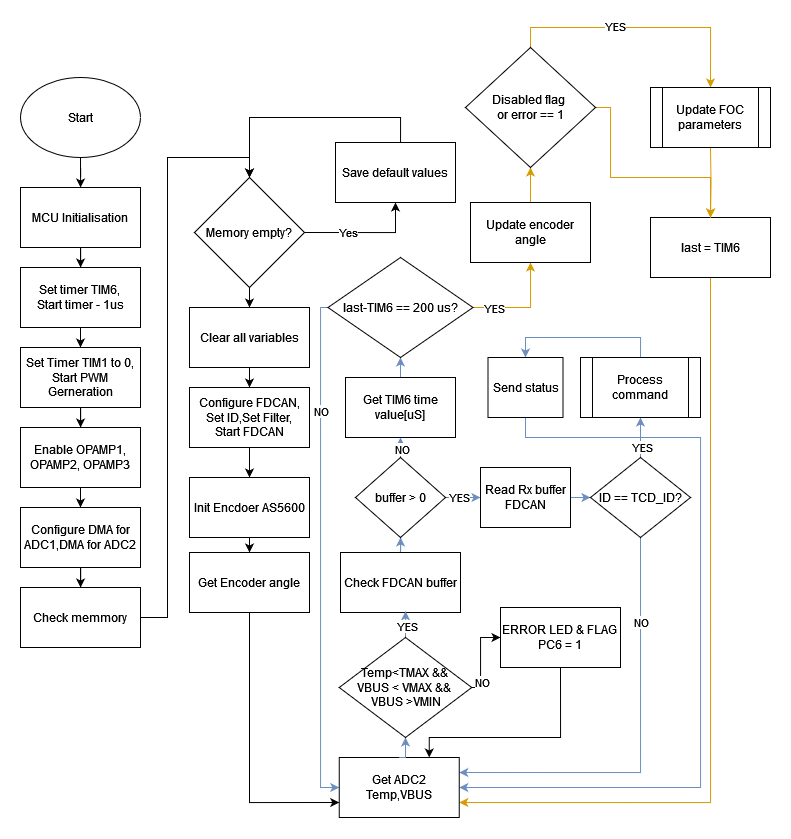
\includegraphics[width=\textwidth]{Src/images/ACD ALG.png}
	\caption{Algorithm of the executive system system.}
	\label{ACDALG}
\end{figure}

Upon power-up, the microcontroller conducts a functionality check of all devices by reading data. The system is divided into two parts: the first part executes functions that do not require frequent execution (highlighted in yellow), and the second part operates at the highest possible frequency, tasks such as computing the vector algorithm and parsing messages are performed in this part, as shown in Figure \ref{ACDCMDALG}.

\begin{figure}[H]
	\centering
	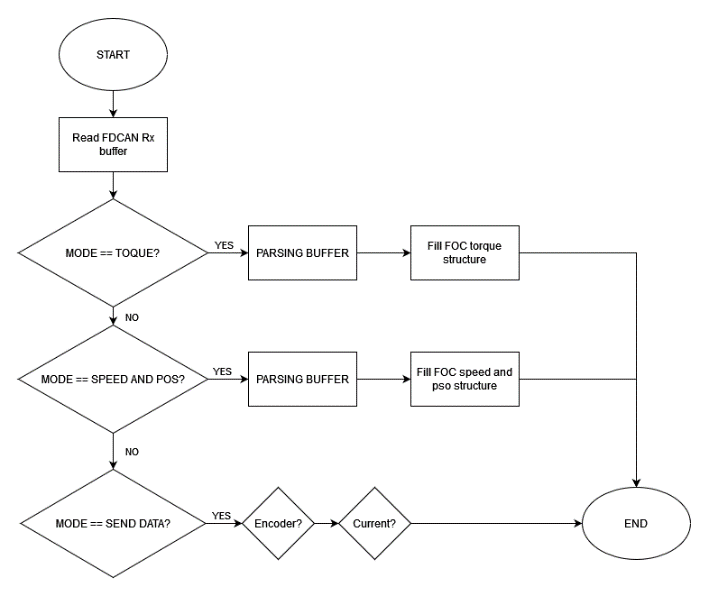
\includegraphics[width=\textwidth]{Src/images/ACDCMDALG.png}
	\caption{Message processing algorithm}
	\label{ACDCMDALG}
\end{figure}

Figure 5.8 illustrates the operation of vector control. As an example, current control with feedback is demonstrated, meaning that the motor always produces a constant torque (i.e., constant current, since torque is proportional to current).

The inputs $i_q$ and $i_d$ are regulated through feedback using a PID controller, which also includes several "Park" and "Clarke" transformation modules. The signals pass through the "SVPWM"  (Space Vector Pulse Width Modulation) block and impact the three-phase inverter to control the motor. The feedback magnitude of the PID controller represents a sampled value of the motor's output current.

\begin{figure}[H]
	\centering
	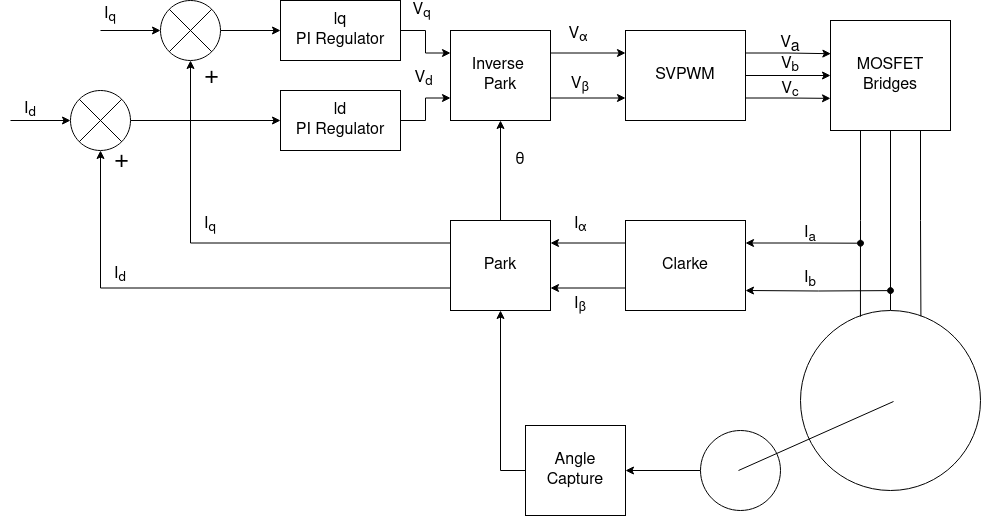
\includegraphics[width=\textwidth]{Src/images/FOC maindrawio.png}
	\caption{Vector motor control diagram.}
	\label{ACDFOCALG}
\end{figure}


The entire vector control process can be broken down into stages:
\begin{enumerate}
\item Acquiring data of the three-phase motor current to compute the values $I_a,I_b$;
\item Converting $I_a,I_b,I_c$ using the Clarke transformation, obtaining $I_\alpha,I_\beta$;
\item Converting $I_\alpha,I_\beta$ using the Park transformation, obtaining $I_q,I_d$;
\item Computing the error of $I_q,I_d$from the set values of $I_q,I_d$coming from the controller;
\item Inputting the specified error into two PID controllers (only PI is used) to get the output control voltages $V_q,V_d$;
\item Converting $V_q,V_d$ using the inverse Park transformation, obtaining $V_\alpha,V_\beta$;
\item Using the space vector $V_\alpha,V_\beta$ to determine the pulse width modulation signals for the three half-bridges of the inverter;
\item Controlling the power MOSFET transistors of the three-phase inverter according to the previously derived code value for motor drive;
\item Repeating the steps mentioned above.
\end{enumerate}

In the calculations, it is sufficient to use the current from only two phases of the motor, as according to Kirchhoff's current law, the third current component can be calculated since the sum of currents flowing into a node is equal to the sum of currents flowing out of the node $I_a+I_b+I_c=0$. The vectors $I_a,I_b,I_c$are not initially orthogonal, and further work requires recalculating the projection into the coordinate axes, formula \ref{Clark}.
\begin{ceqn}
	\begin{align} \label{Clark}
		\begin{cases}
			I_{\alpha} = I_a - \cos\left(\frac{2\pi}{3}\right) I_b - \cos\left(\frac{2\pi}{3}\right) I_c \\
			I_{\beta} = \sin\left(\frac{2\pi}{3}\right) I_b - \sin\left(\frac{2\pi}{3}\right) I_c
		\end{cases}
	\end{align}
\end{ceqn}

After the transformation, a sinusoidal wave is obtained, but with one variable less.The values $I_\alpha, I_\beta$ can be used to control the rotation of the motor, making them correspond to the rules of signal shape change. The inverse Clarke transformation is applied to the three phases of the motor.

The Park transformation, formula \ref{Park}, aims to translate the stationary system $I_\alpha, I_\beta$ into a coordinate system rotating with the rotor $I_q, I_d$, as the system is supposed to receive real-time motor rotation angle data from an encoder. As a result, the rotation vector becomes a fixed value in the $I_\alpha, I_\beta$ coordinate system. Subsequently, $I_q, I_d$ are used as control objects through feedback via a PID controller. In reality, only a PI controller is used, as the differential regulator is omitted, because the transfer function of voltage and current is a first-order inertial element.


\begin{ceqn}
	\begin{align} \label{Park}
		\begin{cases}
			I_d = I_\alpha \cos(\theta) + I_\beta \sin(\theta) \\
			I_q = -I_\alpha \sin(\theta) + I_\beta \cos(\theta)
		\end{cases}
	\end{align}
\end{ceqn}




\begin{figure}[H]
	\centering
	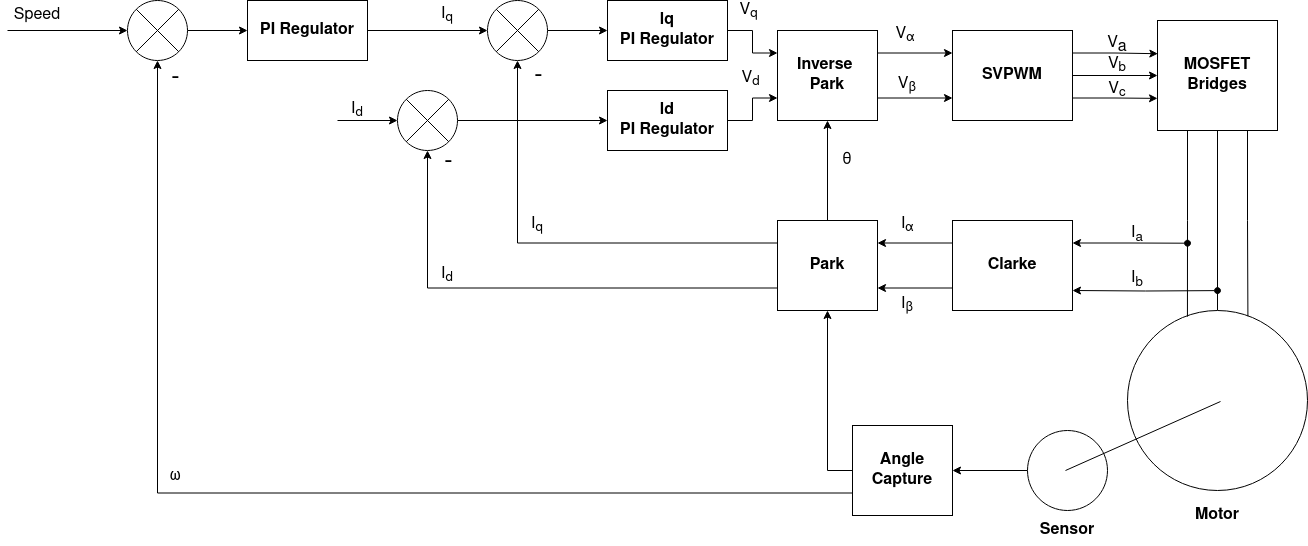
\includegraphics[width=\textwidth]{Src/images/speed.drawio.png}
	\caption{Speed vector motor control scheme}
	\label{ACDFOCALGSPD}
\end{figure}

In standard vector control, three PID loops are primarily used: current loop, speed loop, and position loop. This means controlling the motor current (torque) via current feedback, then controlling the motor speed by managing the torque, and finally controlling the motor position by regulating the speed.

In the figure above \ref{ACDFOCALGSPD}, \(\omega\) is the motor speed feedback, which is calculated using the motor's encoder. It is controlled by a PI regulator.

The calculated motor speed and the speed setpoint value are used to compute the error value, which is then fed into the PI speed loop. The computed result is used as the input signal for the current loop, thus implementing dual speed-current feedback control.

The outermost level is the position loop, which controls the motor by rotating it to a precise angle and maintaining it. The control block diagram is shown in the figure \ref{ACDFOCALGPOS}.


\begin{figure}[H]
	\centering
	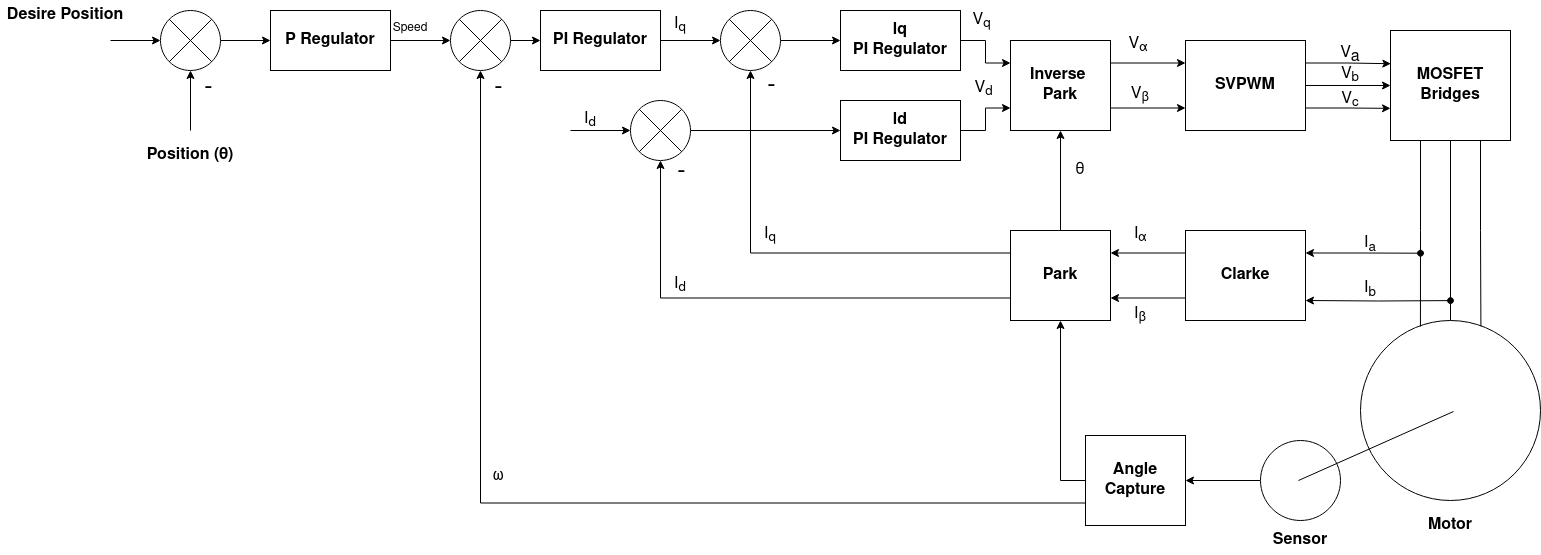
\includegraphics[width=\textwidth]{Src/images/Foc pos.drawio.png}
	\caption{Motor position vector control scheme}
	\label{ACDFOCALGPOS}
\end{figure}


But in the real-world application of the algorithm to a system, the encoder cannot directly return the motor speed. Therefore, the motor speed is calculated by determining the change in encoder value over a specific period of time (i.e., using the average speed to represent the instantaneous speed). This method is suitable when the motor speed is relatively high, but in position control mode, the motor speed will be very low (since the rotor needs to be fixed in a specific position).
To avoid errors caused by speed feedback, only a dual loop consisting of position and current is used for position control. However, at this time, certain modifications need to be made to the position loop as shown in Figure \ref{ACDFOCALGPOSREAL}.

However, it is also taken into account that with the speed loop removed, full PID control is used for the position loop, meaning a differential term is added (since the differential of position is speed, this can reduce position regulation oscillations and speed up convergence, the function of the integral term is to eliminate static error).

\begin{figure}[H]
	\centering
	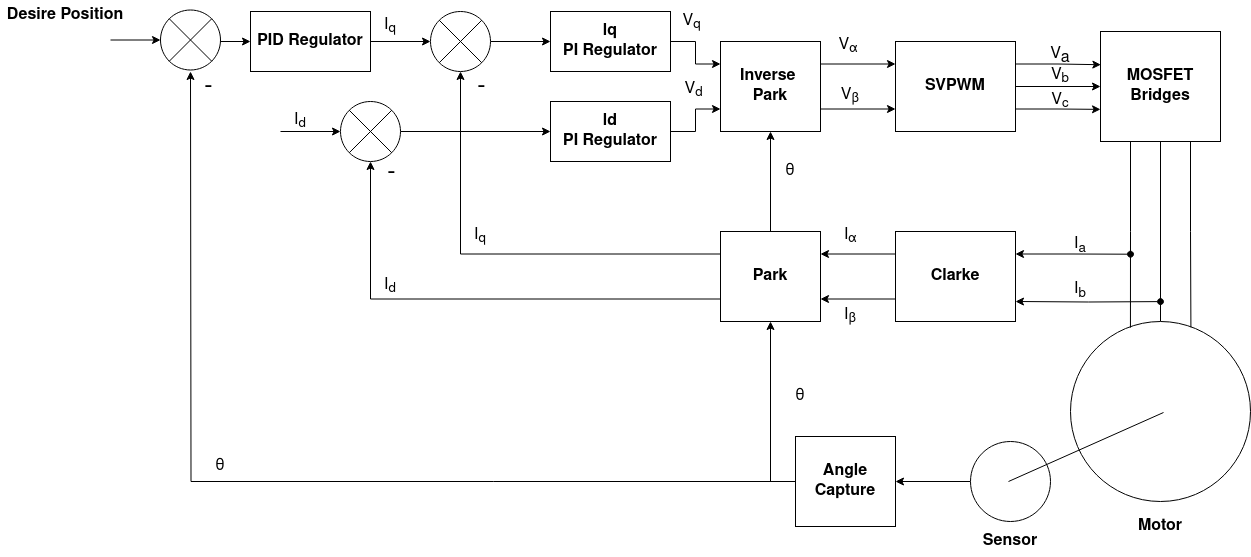
\includegraphics[width=\textwidth]{Src/images/foc pos real.drawio.png}
	\caption{Optimal position vector motor control scheme}
	\label{ACDFOCALGPOSREAL}
\end{figure}



For direct conversion to signals supplied to the power transistors, the SVPWM (Space Vector Pulse Width Modulation) method is used, as it is more efficient than SPWM \citep{Mirdas2023}.


\begin{figure}[H]
	\centering
	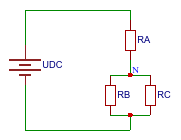
\includegraphics[width=0.3\textwidth]{Src/images/3phasesimpl.png}
	\caption{Equivalent circuit}
	\label{ACDFOC3P}
\end{figure}
To understand the process of signal formation, it is necessary to comprehend the concept of the space voltage vector. The connection of the motor to the voltage source can be visualized as shown in Fig.\ref{ACDFOC3P}.

The three-phase voltages (phase voltage is the voltage of each phase relative to the midpoint of the motor's connection) are expressed by the formula \ref{3ph}:

\begin{ceqn}
	\begin{align} \label{3ph}
		\begin{cases}
			U_a & = U_A - U_N = \frac{2}{3} U_{dc}  \\
			U_b & = U_B - U_N = -\frac{1}{3} U_{dc} \\
			U_c & = U_C - U_N = -\frac{1}{3} U_{dc}
		\end{cases}
	\end{align}
\end{ceqn}
It can be envisioned that the three voltages form vectors \(\vec{U_a}, \vec{U_b}, \vec{U_c}\), which in turn create a resultant vector \(\vec{U}\), enabling the determination of the magnetic field vector. Given that the permanent magnet of the rotor will tend to rotate until the lines of its internal magnetic field align with the direction of the external magnetic field, this vector can effectively represent the direction in which we want the rotor to rotate. Thus, it becomes possible to calculate the space voltage vector \ref{spwm} \citep{youtuFieldOriented}.

\begin{ceqn}
	\begin{align} \label{spwm}
		\begin{cases}
			U_A(t) = U_{dc}\cos(2\pi ft)                             \\
			U_B(t) = U_{dc}\cos\left(2\pi ft - \frac{2\pi}{3}\right) \\
			U_C(t) = U_{dc}\cos\left(2\pi ft + \frac{2\pi}{3}\right)
		\end{cases}
	\end{align}
\end{ceqn}


The SVPWM method synthesises the SPWM value at each time instant\ref{SVPWMF}.
\begin{ceqn}
	\begin{align} \label{SVPWMF}
		\int_0^T U_{\text{ref}} \, dt = \int_0^{T_x} U_x \, dt + \int_{T_x}^{T_x+T_y} U_y \, dt + \int_{T_x+T_y}^T U^*_0 \, dt
	\end{align}
\end{ceqn}

\begin{ceqn}
	\begin{align} \label{SVPWM}
		U_{\text{reference}} \cdot T = U_x \cdot T_x + U_y \cdot T_y + U_0^* \cdot T_0^*
	\end{align}
\end{ceqn}

Thus, the program in the microcontroller uses discretization, which can be simplified to \ref{SVPWM}, where \(U_{\text{reference}}\) is the expected voltage vector, and \(T\) is the PWM period. The essence of the above formula lies in periodically switching between different space voltage vectors, through which an equivalent arbitrary space voltage vector can be synthesized.




\subsection{Software implementation of the actuator control device}
The microcontroller program was developed in C/C++ language, and to facilitate and accelerate development, the HAL (Hardware Abstraction Layer) library was utilized. The set of libraries allows for a higher level of abstraction and enables the porting of code to microcontrollers of a different family. The STM32CubeMX graphical configuration tool was used for project generation and setup. The project was generated for the STM32CubeIDE integrated development environment, which is a modified version of the Eclipse development environment for embedded systems. Figure \ref{STM32G431MX} shows the graphical representation of the clock frequency setting and the clock frequencies of individual peripheral blocks. The microcontroller operates at its maximum frequency, considering the use of an external 8 MHz quartz crystal oscillator. The input frequency is fed into the Phase-Locked Loop (PLL) block, where it undergoes frequency multiplication and division to the output frequency, reaching a level of 94\% of the maximum, i.e., 160 MHz.


\begin{figure}[H]
	\centering
	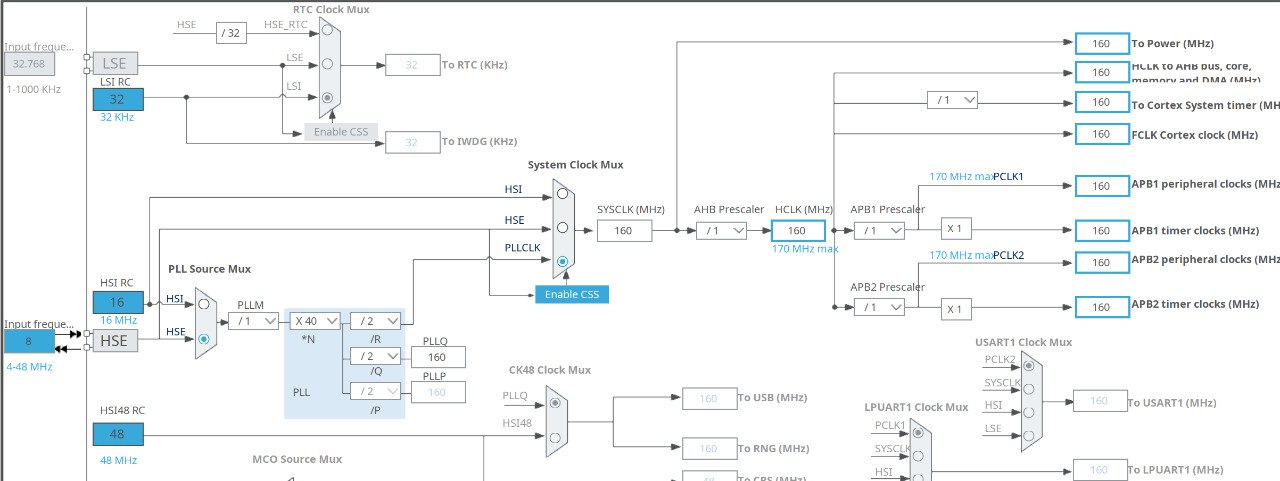
\includegraphics[width=\textwidth]{Src/images/CubeMX.png}
	\caption{STM32G431 microcontroller clocking structure}
	\label{STM32G431MX}
\end{figure}

The encoder is mounted on the motor rotor together with the gearbox, and it was necessary to solve the problem of maintaining the rotation angle. For this purpose, an algorithm for preserving the rotation angle was created for the encoder's rotation range from 0 to 360 degrees. In application 3, a test of the encoder rotation angle algorithm is implemented in Python. To ensure data reading about the rotor's position, the microcontroller sends a data request to the AS5600 encoder, after which a function fills the data structure. A snippet of the function's code is shown in Figure \ref{codeencoder}.



\begin{figure}[H]
	\centering
	\begin{minted}[tabsize=2,breaklines,fontsize=\small]{cpp}
angle_t data;
data.raw = 0;
  if(HAL_I2C_Mem_Read(a->i2cHandle,a->adress,0x0E,I2C_MEMADD_SIZE_8BIT, (uint8_t*)&data.raw,2,2)!= HAL_OK) 
{
  status = HAL_ERROR;
}
  *angle = ((data.bit.angleHIGH << 8) & 0xF00) | data.bit.angleLOW;
}
	\end{minted}
	\caption{Code fragment of the encoder read function}\label{codeencoder}
\end{figure}

The encoder is mounted directly on the shaft of the electric motor. The rotation of the motor exceeds the measurement range of the absolute encoder AS5600 from 0 to 360 degrees (due to the use of a gearbox), necessitating the measurement of the rotation angle in a wider range. The function that measures the current position, speed, and acceleration values is presented in Annex 4.



%\subsection{Алгоритмы устройства тактического управления}



\subsection{Software implementation of the tactical control device}

During various calculations, operations are required that go beyond the standard C++ libraries. Matrix multiplication is often used in calculations, and a function for multiplying two matrices has been implemented, which is shown in Figure \ref{codematrix}. The matrix multiplication function is designed to take three pointers to arrays representing two input matrices and one output matrix, as well as three integer values indicating the sizes of these matrices. The input matrices are referred to as the first and second, and the result of their multiplication is recorded in the output matrix.

To perform matrix multiplication, the function employs three nested loops, where each loop is responsible for its part of the process: the outer loop iterates through the rows of the first matrix, the middle loop through the columns of the second matrix, and the inner loop deals with the elements of the current rows and columns involved in the calculation. This allows the values for each cell of the resulting matrix to be computed sequentially.


\begin{figure}[H]
	\centering
	\begin{minted}[tabsize=2,breaklines,fontsize=\small]{cpp}
    void MultiplyMatrices(const float* matA, const float* matB, float* resultMat, int rowsA, int commonDim, int colsB) {
    float sum;
    int rowIdx, colIdx, kIdx;
    // Loop through each row of the first matrix
    for (rowIdx = 0; rowIdx < rowsA; rowIdx++) {
        // Loop through each column of the second matrix
        for (colIdx = 0; colIdx < colsB; colIdx++) {
            sum = 0.0f; // Temporary variable to store sum
            // Multiply elements across the common dimension
            for (kIdx = 0; kIdx < commonDim; kIdx++) {
                sum += matA[commonDim * rowIdx + kIdx] * matB[colsB * kIdx + colIdx];            }
            // Assign the computed sum to the result matrix
            resultMat[colsB * rowIdx + colIdx] = sum;
        }}}
	\end{minted}
	\caption{Function for multiplication of two matrices}\label{codematrix}
\end{figure}
During the multiplication process, the dot product of the corresponding vectors is calculated for each pair of row and column in the input matrices. To do this, elements of the row from the first matrix are successively multiplied by the corresponding elements of the column from the second matrix, and the results of these multiplications are added together to form the value in the cell of the resulting matrix.

Thus, each element of the output matrix is the sum of the products of the elements of the corresponding row and column of the input matrices, which provides the result of matrix multiplication.

The function for converting a rotation matrix to Euler angles, shown in Figure \ref{codeConvertRotationMatrixToEulerAngles}, takes two arguments: the first argument is a pointer to the input rotation matrix, and the second argument is a pointer to an array where the calculated Euler angles will be stored.


\begin{figure}[H]
	\centering
	\begin{minted}[tabsize=2,breaklines,fontsize=\small]{cpp}
    void ConvertRotationMatrixToEulerAngles(const float* rotationMatrix, float* angles){
        float roll, pitch, yaw, cosPitch;
        if (fabs(rotationMatrix[6]) >= 1.0 - 0.0001){//Check gimbal lock
            roll = 0.0f;  // Set roll to zero as it's indeterminate
            if (rotationMatrix[6] < 0) {// Handle the gimbal lock case
                pitch = (float) M_PI_2;  // 90 degrees
                yaw = atan2f(rotationMatrix[1], rotationMatrix[4]);
            }else{
                pitch = -(float) M_PI_2;  // -90 degrees
                yaw = -atan2f(rotationMatrix[1], rotationMatrix[4]);
            }}else{
            // Regular case, no gimbal lock
            pitch = atan2f(-rotationMatrix[6], sqrtf(rotationMatrix[0] * rotationMatrix[0] + rotationMatrix[3] * rotationMatrix[3]));
            cosPitch = cosf(pitch);
            roll = atan2f(rotationMatrix[3] / cosPitch, rotationMatrix[0] / cosPitch);
            yaw = atan2f(rotationMatrix[7] / cosPitch, rotationMatrix[8] / cosPitch);        }
        angles[0] = yaw;        // Assign calculated angles to output
        angles[1] = pitch;
        angles[2] = roll; }
	\end{minted}
	\caption{Function of matrix transformation into Euler angles}\label{codeConvertRotationMatrixToEulerAngles}
\end{figure}
At the beginning of the function, variables for the three Euler angles: yaw, pitch, and roll, as well as a variable for the cosine of the pitch, are declared. These variables are used to store intermediate calculations and the final results of the conversion.

The function then checks for the condition known as "gimbal lock," which occurs when one of the rotation axes becomes undefined due to the parallelism of the other two axes. The gimbal lock condition is determined by the value of an element in the rotation matrix, and if this value is close to 1 or -1, special processing is performed to calculate the Euler angles.


If the rotation matrix element is less than zero, the pitch angle is set to 90 degrees, and the roll angle is set to zero. The yaw angle is calculated using the arctangent function of two other matrix elements. If the matrix element is not less than zero, the pitch is set to -90 degrees, roll to zero, and yaw is calculated as the negative value of the angle obtained using the arctangent function.

If gimbal lock is not detected, the pitch is calculated through the arctangent of the negative value of the corresponding matrix element and the square root of the sum of the squares of the other two elements. Roll and yaw are then calculated using the cosine of the calculated pitch and the arctangent function for the corresponding matrix elements.

In the end, the calculated yaw, pitch, and roll angle values are stored in the output array in the specified order, completing the conversion of the rotation matrix to Euler angles. The function ConvertEulerAnglesToRotationMatrix is used for the inverse transformation.



The function \textbf{ConvertEulerAnglesToRotationMatrix}, Figure \citep{codeConvertEulerAnglesToRotationMatrix} to convert Euler angles to a rotation matrix takes two pointers to arrays containing the Euler angles (yaw, pitch and roll) and an array for the resulting rotation matrix. At the beginning of the function, variables for the cosines and sines of each of the Euler angles are initialised. These values are calculated to simplify subsequent calculations, as they are used repeatedly in the transformation formulas.

\begin{figure}[H]
	\centering
	\begin{minted}[tabsize=2,breaklines,fontsize=\small]{cpp}
    void ConvertEulerAnglesToRotationMatrix(const float* angles, float* rotationMatrix)
    {
    float cosRoll, cosPitch, cosYaw, sinRoll, sinPitch, sinYaw;
    // Calculate sine and cosine of angles for efficiency
    cosYaw = arm_cos_f32(angles[0]);
    cosPitch = arm_cos_f32(angles[1]);
    cosRoll = arm_cos_f32(angles[2]);
    sinYaw = arm_sin_f32(angles[0]);
    sinPitch = arm_sin_f32(angles[1]);
    sinRoll = arm_sin_f32(angles[2]);

    // Populate the rotation matrix using the sine and cosine values
    rotationMatrix[0] = cosRoll * cosPitch;
    rotationMatrix[1] = cosRoll * sinPitch * sinYaw - sinRoll * cosYaw;
    rotationMatrix[2] = cosRoll * sinPitch * cosYaw + sinRoll * sinYaw;
    rotationMatrix[3] = sinRoll * cosPitch;
    rotationMatrix[4] = sinRoll * sinPitch * sinYaw + cosRoll * cosYaw;
    rotationMatrix[5] = sinRoll * sinPitch * cosYaw - cosRoll * sinYaw;
    rotationMatrix[6] = -sinPitch;
    rotationMatrix[7] = cosPitch * sinYaw;
    rotationMatrix[8] = cosPitch * cosYaw;
    }
	\end{minted}
	\caption{Function of transformation of Euler angles into a matrix}\label{codeConvertEulerAnglesToRotationMatrix}
\end{figure}

Then, using these pre-calculated cosine and sine values, the function fills in the elements of the rotation matrix. The rotation matrix that results from the function is an orthogonal matrix that describes rotation in three-dimensional space. 

The main task of the tactical device is to calculate the trajectory of the robot, in order to provide this we have written functions to solve the forward or inverse kinematic problem for a 6-axis mini robot, the code is presented in \textbf{Annex 6}. 

The function "CalculateFK" is designed to determine the position and orientation of the final actuator of a robot with six degrees of freedom based on the given rotation angles of its links. Then, for each link, a rotation matrix is calculated based on its rotation angle and parameters specified in the Denavit-Hartenberg table. These parameters describe the mutual arrangement of the robot links. The rotation matrix of all links is multiplied sequentially from the base of the robot to its final actuator. This multiplication gives the total rotation matrix, which describes the complete orientation and position of the final actuator relative to the robot base.
By summing the position vectors of all links, the function finds the final position of the robot's final actuator.
In the final step, based on the total rotation matrix, the function calculates Euler angles that describe the orientation of the final actuator in space. These angles represent rotation around three axes and allow the exact orientation of the actuator to be determined. The results of the calculations - the coordinates of the position of the actuator and its orientation - are written to the output structure \textbf{outputPose}.

The most complex function is the solution of the inverse kinematics problem, which, based on the rotation matrix, calculates three angles: yaw, pitch and roll. For yaw and pitch, the calculations are based on rotations around the vertical and horizontal axes, respectively, while roll is determined through rotation around the gaze axis. The calculations take into account the physical limitations of the joints to ensure that the resulting angles are realistic and feasible. The results, represented as yaw, pitch and roll angles, are then written to a designated array, ready to be used to control the robot's movements. The boolean value returned by the function serves as an indicator of the success of the operation: true indicates that the angles have been successfully calculated and are within acceptable values, while false indicates that the required orientation cannot be achieved due to constraints imposed by the joint design.